% WCCM talk: NEML2 nodal-force interface for explicit dynamics in MOOSE
% Scaffold (Claude). Compile:  latexmk -pdf WCCM_NEML2_explicit_dynamics.tex
% Speaker notes: uncomment the \setbeameroption line below to show \note{} content.
\documentclass[aspectratio=169,11pt]{beamer}
\usepackage{amsmath,amssymb}
\usepackage{graphicx}
\usepackage{tikz}
\usetikzlibrary{positioning,arrows.meta,calc}
\usepackage{xcolor}
\graphicspath{{./}}

\definecolor{navy}{HTML}{1B2A4A}
\definecolor{nblue}{HTML}{1F77B4}
\definecolor{ngreen}{HTML}{2CA02C}
\definecolor{nred}{HTML}{C0392B}
\definecolor{ngold}{HTML}{B9770E}

\usetheme{default}
\setbeamertemplate{navigation symbols}{}
\setbeamercolor{structure}{fg=nblue}
\setbeamercolor{frametitle}{fg=navy}
\setbeamerfont{frametitle}{series=\bfseries,size=\large}
\setbeamertemplate{frametitle}{%
  \vspace*{0.4em}\insertframetitle\\[-0.2em]{\color{nblue}\rule{0.18\textwidth}{1.2pt}}}
\setbeamertemplate{itemize item}{\color{nblue}\textbullet}
\setbeamertemplate{footline}{\hfill{\color{gray}\scriptsize\insertframenumber/\inserttotalframenumber}\hspace{2mm}\vspace{1mm}}
% \setbeameroption{show notes}            % <- uncomment to render speaker notes

\newcommand{\Rint}{\mathbf{R}_{\mathrm{int}}}
\newcommand{\Fext}{\mathbf{F}_{\mathrm{ext}}}

\title{GPU-resident material evaluation for explicit dynamics}
\subtitle{A NEML2--MOOSE nodal-force interface}
\author{Author Name \and Co-authors}
\institute{Idaho National Laboratory / \ldots}
\date{WCCM 2026 \quad\textbar\quad [session] \quad\textbar\quad [date]}

\begin{document}

% ===== 1 TITLE =====
{\setbeamertemplate{footline}{}\begin{frame}[plain]\titlepage\end{frame}}
\note{SPINE = method/architecture-first: the NEML2--MOOSE explicit coupling is the contribution; the Taylor slug is the proof; verification vs MOOSE J2 is the credibility check. ~15 slides / 20 min. Audience: general comp-mech, MOOSE/NEML2-naive.}

% ===== 2 THE GAP =====
\begin{frame}{The capability gap}
\begin{itemize}
  \item MOOSE: mature \emph{implicit} multiphysics --- boundary conditions, contact, parallel domain decomposition
  \item Missing: GPU-accelerated \emph{explicit} dynamics driven by modern (auto-differentiated, tensor) constitutive models
  \item High-rate events (impact, blast; advanced-reactor safety) are bottlenecked by per-point material evaluation
  \item \textbf{This talk:} how we closed that gap --- and kept MOOSE's infrastructure
\end{itemize}
\end{frame}
\note{HOOK = capability-gap-first (chosen). Add ONE sentence of broader stakes so a non-MOOSE attendee cares. Reactors = the high-consequence application, not the whole pitch.}

% ===== 3 MOOSE =====
\begin{frame}{MOOSE --- multiphysics finite-element framework}
\begin{itemize}
  \item Open-source FE framework for coupled multiphysics (INL)
  \item Robust infrastructure: BCs, contact, parallel domain decomposition, adaptivity
  \item Strong implicit-solver heritage (Newton $+$ PETSc)
  \item Extensible: physics added as modular C\texttt{++} objects
\end{itemize}
\end{frame}
\note{Audience is MOOSE-naive --- keep to ~1 min. Just enough that ``we extended MOOSE'' lands.}

% ===== 4 NEML2 =====
\begin{frame}{NEML2 --- tensor constitutive-model library}
\begin{itemize}
  \item Constitutive models composed from small reusable operators
  \item Automatic differentiation $\Rightarrow$ exact consistent Jacobians
  \item libTorch (PyTorch C\texttt{++}) backend $\Rightarrow$ device-independent: CPU / CUDA / MPS
  \item Batched evaluation: all material points as \emph{one} tensor operation
\end{itemize}
\end{frame}
\note{The ``GPU-capable, batched, AD'' points set up the whole method. Device-independence is real in code (torch::Device plumbing).}

% ===== 5 WHY EXPLICIT =====
\begin{frame}{Why explicit dynamics}
\begin{itemize}
  \item High-rate regime: impact, wave propagation, short timescales
  \item No global linear/nonlinear solve --- march node-by-node
  \item Conditionally stable: timestep bounded by CFL ($\Delta t \le \Delta t_{\mathrm{crit}}$)
  \item Lumped (diagonal) mass $\Rightarrow$ trivial $\mathbf{M}^{-1}$; cost shifts to the constitutive update
  \item $\Rightarrow$ making the material model fast is the whole game
\end{itemize}
\end{frame}
\note{Frames the contribution: in explicit dynamics the per-element constitutive evaluation dominates, so GPU-resident batched evaluation is the lever.}

% ===== 6 CONTRIBUTION =====
\begin{frame}{Contribution --- two pillars}
\begin{itemize}
  \item[\textcolor{nblue}{\textbf{1.}}] \textcolor{nblue}{\textbf{ExplicitMixedOrder}}: a mixed-order explicit time integrator (our work, MOOSE \texttt{solid\_mechanics})
  \item[\textcolor{nblue}{\textbf{2.}}] \textcolor{nblue}{\textbf{NEML2 nodal-force path}}: internal forces assembled \emph{inside} NEML2
  \begin{itemize}
    \item \texttt{NEML2StressDivergence} $+$ NEML2 interpolation/assembly userobjects
    \item constitutive state kept resident in NEML2 between steps
  \end{itemize}
  \item[\textcolor{ngreen}{$\hookrightarrow$}] built on MOOSE's existing BC / contact / parallel-DD infrastructure
\end{itemize}
\end{frame}
\note{ATTRIBUTION (verified): ExplicitMixedOrder authored by us (2025-04, now upstreamed); NEML2 force path by the team (2025-06). BOTH built for this project. Name it ExplicitMixedOrder, NOT ``central difference'' (the generic CentralDifference predates us). MOOSE+NEML2 talk; do NOT introduce Marlin.}

% ===== 7 FORMULATION (native math) =====
\begin{frame}{Formulation}
\begin{align*}
\mathbf{M}\,\ddot{\mathbf{u}} &= \Fext - \Rint
   &&\text{\footnotesize semi-discrete momentum (lumped $\mathbf{M}$)}\\[4pt]
\Rint &= \bigcup_{e}\int_{\Omega_e}\!\nabla\phi : \boldsymbol{\sigma}\,dV,
   \quad \boldsymbol{\sigma}=\mathcal{N}_{\theta}(\boldsymbol{\varepsilon})
   &&\text{\footnotesize $\mathcal{N}_\theta$: NEML2 model (AD, GPU-capable)}\\[4pt]
\ddot{\mathbf{u}}^{\,n} &= \mathbf{M}^{-1}\!\big(\Fext^{\,n}-\Rint^{\,n}\big),
   \quad \mathbf{u}^{n+1}=2\mathbf{u}^{n}-\mathbf{u}^{n-1}+\Delta t^2\ddot{\mathbf{u}}^{\,n}
   &&\text{\footnotesize central diff. (ExplicitMixedOrder)}
\end{align*}
\vspace{0.5em}
\begin{center}
\setbeamercolor{block body}{bg=ngold!12}
\fcolorbox{ngold}{ngold!10}{\parbox{0.8\textwidth}{\centering\textbf{The entire $\Rint$ assembly is \emph{one} batched tensor evaluation in NEML2.}}}
\end{center}
\end{frame}
\note{Core figure framing = weak-form equation-first (chosen). Punchline: R\_int assembly is ONE batched NEML2 tensor op.}

% ===== 8 FORCE PATH (TikZ) =====
\begin{frame}{Nodal forces assembled inside NEML2}
\begin{center}
\resizebox{\linewidth}{!}{%
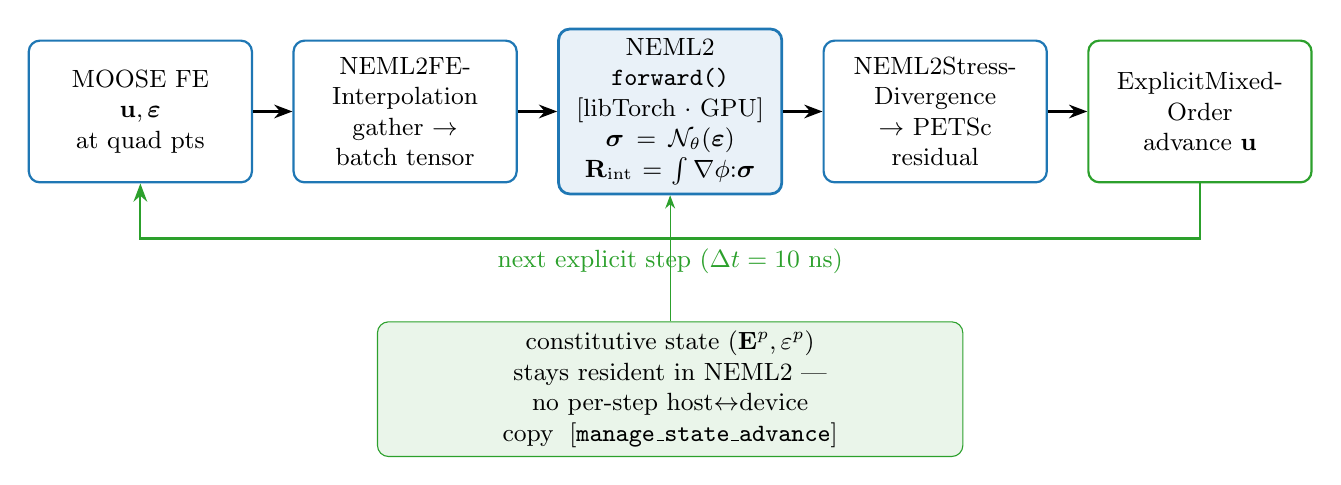
\begin{tikzpicture}[>=Stealth, node distance=5mm,
   b/.style={draw=nblue, thick, rounded corners, align=center, minimum height=18mm, text width=26mm, font=\small}]
  \node[b] (a) {MOOSE FE\\$\mathbf{u},\boldsymbol{\varepsilon}$\\at quad pts};
  \node[b, right=of a] (i) {NEML2FE-\\Interpolation\\gather $\to$ batch tensor};
  \node[b, right=of i, fill=nblue!10, line width=1pt] (c) {NEML2 \texttt{forward()}\\ {[}libTorch $\cdot$ GPU{]}\\$\boldsymbol{\sigma}=\mathcal{N}_\theta(\boldsymbol{\varepsilon})$\\$\mathbf{R}_{\mathrm{int}}=\int\nabla\phi{:}\boldsymbol{\sigma}$};
  \node[b, right=of c] (d) {NEML2Stress-\\Divergence\\$\to$ PETSc residual};
  \node[b, right=of d, draw=ngreen] (e) {ExplicitMixed-\\Order\\advance $\mathbf{u}$};
  \draw[->,thick] (a)--(i); \draw[->,thick] (i)--(c); \draw[->,thick] (c)--(d); \draw[->,thick] (d)--(e);
  \draw[->,thick,ngreen] (e.south) -- ++(0,-7mm) -| (a.south)
       node[pos=0.25, below, font=\small] {next explicit step ($\Delta t=10$ ns)};
  \node[draw=ngreen, fill=ngreen!10, rounded corners, align=center, font=\small,
        below=16mm of c, text width=72mm] (note)
     {constitutive state $(\mathbf{E}^p,\varepsilon^p)$ stays resident in NEML2 --- \\
      no per-step host$\leftrightarrow$device copy \;[\texttt{manage\_state\_advance}]};
  \draw[->,ngreen] (note) -- (c);
\end{tikzpicture}}
\end{center}
\end{frame}
\note{The actual novelty: NEML2StressDivergence::forward() builds the residual in libTorch under torch::InferenceMode and add\_vector()'s into PETSc. Code: moose/modules/solid\_mechanics/src/neml2/NEML2StressDivergence.C:57-88.}

% ===== 9 STATE RESIDENCY (TikZ) =====
\begin{frame}{No per-step state transfer}
\begin{center}
\resizebox{0.78\linewidth}{!}{%
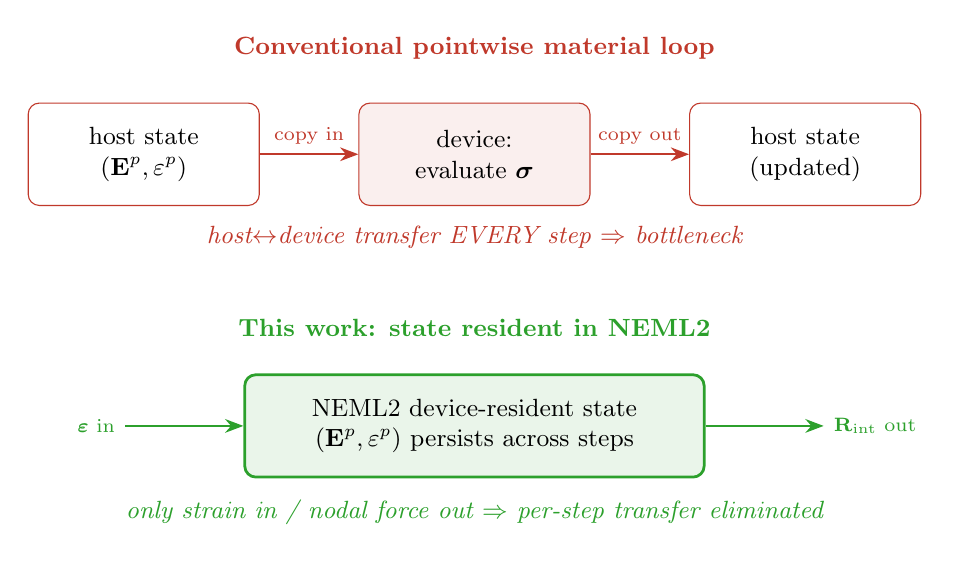
\begin{tikzpicture}[>=Stealth,
   r/.style={draw=nred, rounded corners, align=center, minimum height=13mm, text width=27mm, font=\small},
   g/.style={draw=ngreen, rounded corners, align=center, minimum height=13mm, font=\small}]
  % conventional
  \node[font=\bfseries\small, nred] at (4.2,1.35) {Conventional pointwise material loop};
  \node[r] (h1) at (0,0) {host state\\$(\mathbf{E}^p,\varepsilon^p)$};
  \node[r, fill=nred!8] (dv) at (4.2,0) {device:\\evaluate $\boldsymbol{\sigma}$};
  \node[r] (h2) at (8.4,0) {host state\\(updated)};
  \draw[->,thick,nred] (h1)--(dv) node[midway,above,font=\scriptsize]{copy in};
  \draw[->,thick,nred] (dv)--(h2) node[midway,above,font=\scriptsize]{copy out};
  \node[nred, font=\itshape\small] at (4.2,-1.05) {host$\leftrightarrow$device transfer EVERY step $\Rightarrow$ bottleneck};
  % this work
  \node[font=\bfseries\small, ngreen] at (4.2,-2.2) {This work: state resident in NEML2};
  \node[g, fill=ngreen!10, line width=1pt, text width=56mm] (res) at (4.2,-3.45)
     {NEML2 device-resident state $(\mathbf{E}^p,\varepsilon^p)$ persists across steps};
  \draw[<-,thick,ngreen] (res.west) -- ++(-1.5,0) node[left,font=\scriptsize]{$\boldsymbol{\varepsilon}$ in};
  \draw[->,thick,ngreen] (res.east) -- ++(1.5,0) node[right,font=\scriptsize]{$\mathbf{R}_{\mathrm{int}}$ out};
  \node[ngreen, font=\itshape\small] at (4.2,-4.55) {only strain in / nodal force out $\Rightarrow$ per-step transfer eliminated};
\end{tikzpicture}}
\end{center}
\end{frame}
\note{manage\_state\_advance=true keeps (Ep, ep) resident in NEML2. The efficiency lever. Keep the precise object graph as a Q\&A backup.}

% ===== 10 PERFORMANCE =====
\begin{frame}{Performance: material-evaluation throughput}
\begin{itemize}
  \item Frame around throughput: material-point evaluations / second on the device
  \item Where does the bottleneck move once material eval is GPU-resident?
  \item Roofline view: batched constitutive kernel vs.\ memory traffic
\end{itemize}
\vspace{1em}
\begin{center}
\fcolorbox{ngold}{ngold!8}{\parbox{0.82\textwidth}{\centering\vspace{6mm}
  \textbf{[ insert throughput / roofline plot ]}\\[2mm]
  {\color{nred}$\triangle$ NEEDS a real GPU run $+$ elements/s instrumentation}\vspace{6mm}}}
\end{center}
\end{frame}
\note{ACTION ITEM (heaviest open): every impact run is compute\_devices='cpu' today --- no GPU run, no timing. Perf framing chosen = roofline/throughput. Must measure before the talk; else fall back to a qualitative architecture argument labelled in-progress.}

% ===== 11 SETUP =====
\begin{frame}{3D Taylor anvil impact --- setup}
\begin{itemize}
  \item OFHC copper slug: 0.3 in dia.\ $\times$ 1.5 in, flat-on impact at 235.9 m/s
  \item ExplicitMixedOrder $+$ NEML2 Johnson--Cook (inverted form), $\Delta t = 10$ ns
  \item JC params: $A{=}99.7$, $B{=}262.8$ MPa, $n{=}0.23$, $C{=}0.029$, $m{=}0.98$
  \item Rigid wall: penalty Neumann BC \emph{(architecture compatible with MOOSE contact --- future)}
\end{itemize}
\end{frame}
\note{CONTACT (decision): forward ``compatible with MOOSE contact'' claim ONLY --- not demonstrated. Anvil is a penalty FunctionNeumannBC; CONTACT module off. Backup for ``show me'': the force path plugs into MOOSE contact unchanged; demo is future work.}

% ===== 12 VERIFICATION =====
\begin{frame}{Verification vs MOOSE native J2}
\begin{center}\includegraphics[width=0.9\linewidth]{verification_2d_matched.png}\end{center}
\vspace{-0.3em}
{\footnotesize Matched constitutive (NEML2 vs MOOSE radial-return J2) isolates the force-assembly implementation:
forces agree to $3.8\times10^{-4}$, displacement to $3\times10^{-8}$.}
\end{frame}
\note{WORDING FIX (decision): ``verified against MOOSE's native J2 stress update'' --- NOT ``vs implicit''. Committed comparison is explicit-vs-explicit. A 3D dynamic-history companion (verification.png) exists but mixes J2-vs-JC models (label model-to-model, peak L2 ~3.6\%).}

% ===== 13 RESULTS =====
\begin{frame}{3D Taylor impact --- results}
\begin{columns}[T]
  \begin{column}{0.58\textwidth}\includegraphics[width=\linewidth]{demo_mushroom_pstrain.png}\end{column}
  \begin{column}{0.42\textwidth}\includegraphics[width=\linewidth]{demo_mushroom_profile.png}\end{column}
\end{columns}
\vspace{0.3em}
{\footnotesize Plastic strain localizes at the impact foot (peak $\approx 0.44$); deformed profile shows
full-hard 51\% vs annealed 58\% axial shortening (temper sensitivity captured).}
\end{frame}
\note{Demo visual (decision) = static field snapshots. Validation vs experimental STL is INTENTIONALLY OUT (sim under-predicts mushroom flare ~36\%). Present as capability demo, not validation.}

% ===== 14 THERMOMECHANICAL =====
\begin{frame}{Coupled thermomechanical: temperature from plastic work}
\begin{itemize}
  \item Adiabatic Taylor--Quinney heating: $\rho c_p \dot{T} = \beta\,\sigma_{vm}\,\dot{\varepsilon}_p$ \;($\beta\approx0.9$)
  \item Integrated \emph{inside} NEML2 --- no heat-conduction PDE, no extra module
  \item Justified: diffusion length $\sqrt{\alpha t}\approx 0.11$ mm $\ll$ element ($\sim$2 mm) over 120 $\mu$s
  \item Expected peak $\Delta T \approx 40$--$50$ K at the mushroom ($\approx 3$--$4\%$ softening)
\end{itemize}
\vspace{0.5em}
\begin{center}
\fcolorbox{ngold}{ngold!8}{\parbox{0.86\textwidth}{\centering\vspace{3mm}
  \textbf{[ insert temperature-field snapshot ]}\\[1mm]
  {\color{nred}$\triangle$ NEEDS the coupled run --- see \texttt{johnson\_cook\_neml2\_thermal.i} $+$ scoping doc}\vspace{3mm}}}
\end{center}
\end{frame}
\note{ACTION ITEM: generate the coupled run (draft input + scoping doc in slide\_assets/). Runtime risk: initialize old\_state/T to 300 K. Wording: ``adiabatic temperature rise from plastic work''. Don't oversell --- ~40 K is real but secondary at this velocity.}

% ===== 15 CONCLUSIONS =====
\begin{frame}{Conclusions \& future work}
\begin{itemize}
  \item \textcolor{nblue}{\textbf{Contribution}}: ExplicitMixedOrder integrator $+$ NEML2 nodal-force path
  \item GPU-resident, batched material evaluation; state stays in NEML2 (no per-step transfer)
  \item Verified against MOOSE native J2 (forces to $10^{-4}$); 3D Taylor impact demonstrated
  \item \textcolor{ngreen}{\textbf{Future work:}}
  \begin{itemize}
    \item GPU throughput at scale \quad $\bullet$ integration with MOOSE contact
    \item Bayesian calibration / UQ of constitutive parameters \quad $\bullet$ experimental validation
  \end{itemize}
\end{itemize}
\end{frame}
\note{Recap two pillars $+$ efficiency lever. Future-work bullets absorb the items cut from this talk (UQ/Bayesian, validation, contact) so the abstract's full scope is acknowledged as roadmap.}

\end{document}
